\subsection{Specific Privacy}

In addition to the Zcash\cite{website:Zcash} team, the public blockchain that implements private transactions 
include Monero\cite{website:Monero}, Dash\cite{website:Dash}, Grin\cite{website:Grin}, etc, but these public chains do not have any 
programmability and can only be used for private transfer of assets, so compared to 
Ethereum\cite{website:Ethereum}, ecological development is much behind. Similarly, Ethereum\cite{website:Ethereum} has become 
the largest public chain in the ecosystem so far because of its programmability, 
but there is no privacy. Therefore, some projects have begun to try to bring privacy to 
Ethereum\cite{website:Ethereum}, such as ZK-ZKRollup application zk.money\cite{website:zk.money}, developed by the Aztec\cite{website:Aztec} team. 
but the current zk.money\cite{website:zk.money} product is sunset, the main reason is that zk.money\cite{website:zk.money}
the same can only be applied to a single privacy transfer scenario. Under the premise 
of the current Defi application explosion, a transfer is only one of the simplest 
financial Scenarios, therefore, the user base is not high, but it has to continue 
to pay maintenance costs.
\begin{figure}[!ht]
    \centering
    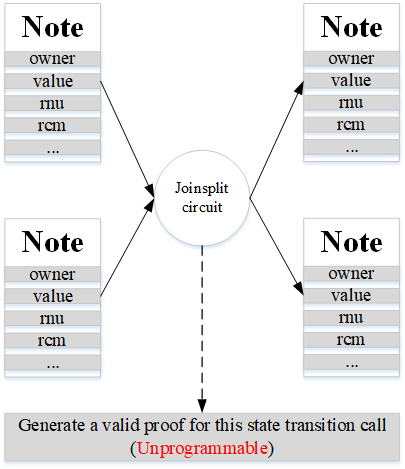
\includegraphics[width=0.4\textwidth]{Example of Specific privacy.jpg}
    \caption{Example of Specific privacy}
    \label{fig:Example of Specific privacy}
\end{figure}

Figure \ref{fig:Example of Specific privacy} shows the simple logic of specific privacy. Since the scene is single(most of 
they are privacy transfers), the value change logic corresponding to the input and output 
notes are also fixed, generally in the form of `A + B = C + D`. The Manta network\cite{website:Manta-network} is a 
layer1 that supports user-defined token privacy transfers, and the privacy transaction 
constraint circuits of all fungible tokens can be used to reuse the above logic.

The ZK-ZKRollup application of a single scene is like the ZKRollup application of a 
single scene. If you want to use the asset for 
other scenarios, you must cross the asset to another application through a bridge, 
which is very unfriendly to the user experience. Therefore, just as ZKRollup needs to 
transition to ZK(E)VM, ZK-ZKRollup also needs to transition to ZK-ZKVM (Appendix \ref{section:appendix} explains 
how to get solidity compatibility).